\section{Language Definition}
\label{sec:language}

\definecolor{ltloEtype}{RGB}{214,230,245}
\definecolor{ltloAttr}{RGB}{220,240,214}
\definecolor{ltloRel}{RGB}{245,220,220}

This section reports the second iTelos phase. Its input is the formal purpose of Section~3 and the data sources collected in the Information Gathering (Section~\ref{sec:info-gathering}); its output is the language of the KG. The phase works on two layers. In the knowledge layer we fixed the terms for entity types, object properties and data properties, and aligned each of them to a Language Teleontology (LTLO). In the data layer we filtered, cleaned and formatted the datasets so that their columns and values use the same terms. The design material is in the folder \texttt{Phase 2 - Language Definition/}; the scripts are in \texttt{Phase 4 - Entity Definition/src/} and their outputs in \texttt{Phase 4 - Entity Definition/data/processed/}.

\subsection{Knowledge Layer}

\subsubsection{Fixing Language Terms}

We started from every term of the Purpose ER model (Figure~\ref{fig:er}) and gave each one its final English name. Three conventions were fixed before starting:
\begin{itemize}
    \item \textbf{Namespace.} The terms live in the namespace \texttt{http://knowdive.disi.unitn.it/etype\#}, as in the course examples, with the prefix \texttt{tpkg:} (Transcriptomics Pathways KG).
    \item \textbf{Naming.} Classes are written in UpperCamelCase (\texttt{tpkg:CellType}), object and data properties in lowerCamelCase (\texttt{tpkg:isMarkerFor}, \texttt{tpkg:approvedSymbol}), without a \texttt{has} prefix.
    \item \textbf{Custom concepts.} Concepts defined by the project get the identifiers \texttt{TPKG26-01}, \texttt{TPKG26-02}, \ldots
\end{itemize}

\noindent The four entity types and the five object properties kept their Phase~1 meaning and were only renamed to the convention (e.g.\ \emph{participates in} $\rightarrow$ \texttt{tpkg:participatesIn}). For the data properties four changes were made:
\begin{itemize}
    \item \textbf{One label for all.} Pathway and Disease both had a \emph{label}. Instead of a new term we reuse the standard \texttt{rdfs:label}, the usual way to give a resource a readable name. The two Phase~1 labels therefore become one term.
    \item \textbf{Singular names for multi-valued properties} (\texttt{tpkg:sourceSymbol}, \texttt{tpkg:sourceDiseaseName}). In RDF each triple carries one value, so a gene with three source symbols has three \texttt{tpkg:sourceSymbol} triples, each read as ``has source symbol X''. Whether a property can have more than one value is not part of its name.
    \item \textbf{\texttt{tpkg:sourceDiseaseName}} instead of \emph{source strings}: the values are the disease names as CellMarker writes them; ``strings'' only described the data type.
    \item \textbf{\texttt{tpkg:hgncResolutionMethod}} instead of \emph{resolution status}. In the data layer we decided that only genes with an HGNC identifier enter the KG (decision D21 below), so the attribute can only say \emph{how} a gene was resolved (on the approved symbol, or on a unique previous or alias symbol). It was renamed and its gloss changed accordingly.
\end{itemize}
The four evidence attributes of \emph{is marker for} (marker source, method details, PubMed ID, publication year) had already been removed at the end of Phase~1; they are counted as initially considered and not finally considered.

\subsubsection{Language Teleontology Alignment}

\noindent\textbf{Reference LTLO and search order.} The guide lets each team choose its reference LTLO. Following the Oncovirus KG example, we used three tiers. For each term we looked first in the \textbf{UKC} (Universal Knowledge Core) \cite{giunchiglia2017understanding}, the lexical resource developed at KnowDive. If the UKC had no concept with a fitting sense, we looked in the \textbf{biomedical ontologies} of the project proposal and of the OBO Foundry / NCBO BioPortal, read through EBI OLS. Only when neither had a suitable concept did we define a \textbf{new concept} with a \texttt{TPKG26} identifier, placed under the closest existing concept. A UKC concept was skipped only when its sense was too generic for the biological relation, and the reason is recorded. Every identifier and gloss was checked on its source on 2026-11-18 (Table~\ref{tab:ltlo-resources}).

\begin{table}[htbp]
\centering
\small
\begin{tabularx}{\linewidth}{|l|X|l|}
\hline
\textbf{Resource} & \textbf{Version and access} & \textbf{Used for} \\ \hline
UKC \cite{giunchiglia2017understanding} & \texttt{ukc.datascientia.eu} & 3 terms, 5 parents \\ \hline
NCI Thesaurus (NCIt) \cite{sioutos2007nci} & 26.02d (release 2026-03-19), via EBI OLS & 2 terms \\ \hline
Experimental Factor Ontology (EFO) \cite{malone2010modeling} & v3.96.0, via EBI OLS & 1 term \\ \hline
Relation Ontology (RO) \cite{smith2005relations} & release 2026-09-04, via EBI OLS & 2 terms \\ \hline
EDAM \cite{ison2013edam} & 1.25 (2026-06-26), via EBI OLS & 9 terms \\ \hline
W3C RDF Schema & namespace \texttt{rdfs:} & \texttt{rdfs:label} \\ \hline
\end{tabularx}
\caption{Resources used for the language alignment}
\label{tab:ltlo-resources}
\end{table}

\noindent\textbf{Alignment per entity type.} Following the example report, for each entity type we give the alignment of the class and of its attributes.

\begin{enumerate}
    \item \textbf{Class: Gene.}
    \begin{itemize}
        \item \emph{Alignment:} UKC-29340 \emph{gene} (parent UKC-44849 \emph{sequence}). The UKC gloss describes a protein-coding gene, while our genes, taken from HGNC, also include non-coding genes and pseudogenes; the word is the same, so the alignment holds at the language level.
        \item \emph{Attribute mapping:} \texttt{hgncId} $\rightarrow$ EDAM:data\_2298 \emph{Gene ID (HGNC)}; \texttt{approvedSymbol} $\rightarrow$ NCIT:C43568 \emph{Gene Symbol}, whose gloss says ``approved by a nomenclature committee''; \texttt{approvedName} $\rightarrow$ EDAM:data\_2299 \emph{Gene name}; \texttt{sourceSymbol} $\rightarrow$ EDAM:data\_1026 \emph{Gene symbol}, the generic concept, because a source symbol may be a previous or alias symbol; \texttt{hgncResolutionMethod} $\rightarrow$ new concept TPKG26-04 (parent UKC-38540 \emph{result}).
    \end{itemize}
    \item \textbf{Class: Pathway.}
    \begin{itemize}
        \item \emph{Alignment:} NCIT:C54214 \emph{Pathway}. The UKC has \emph{pathway} only as a trodden path (UKC-21030) or a nerve pathway (UKC-29542). Among the ontology candidates (PW:0000001, NCIT:C54214, NCIT:C20633 \emph{Biochemical Pathway}) we chose the broadest one: a Hallmark gene set groups the genes of a biological state or process, not necessarily a sequence of reactions.
        \item \emph{Attribute mapping:} \texttt{hallmarkId} $\rightarrow$ EDAM:data\_1082 \emph{Pathway or network identifier} (EDAM has identifiers for several pathway databases, but none for MSigDB); \texttt{rdfs:label} reused as it is; \texttt{sourceUrl} $\rightarrow$ EDAM:data\_1052 \emph{URL}.
    \end{itemize}
    \item \textbf{Class: CellType.}
    \begin{itemize}
        \item \emph{Alignment:} EFO:0000324 \emph{cell type}. The UKC has \emph{cell} (UKC-34) but not \emph{cell type}. Our CellType is qualified by its context (cell name, tissue class, disease category), which the gloss does not cover.
        \item \emph{Attribute mapping:} \texttt{cellName} $\rightarrow$ EDAM:data\_2892 \emph{Cell type name}; \texttt{tissueType} $\rightarrow$ UKC-28479 \emph{tissue} (its values are tissue names); \texttt{cellOntologyId} $\rightarrow$ EDAM:data\_3238 \emph{Cell type ontology ID}; \texttt{tissueClass}, \texttt{diseaseCategory} and \texttt{cellNameClass} $\rightarrow$ new concepts TPKG26-05, TPKG26-06 and TPKG26-07, because they are groupings defined by CellMarker itself.
    \end{itemize}
    \item \textbf{Class: Disease.}
    \begin{itemize}
        \item \emph{Alignment:} UKC-67092 \emph{disease} (parent UKC-67044 \emph{illness}). The instances are MONDO terms; aligning the class to the MONDO root is a knowledge-layer choice left to Phase~3.
        \item \emph{Attribute mapping:} \texttt{mondoId} $\rightarrow$ EDAM:data\_3667 \emph{Disease identifier}; \texttt{rdfs:label} reused as it is; \texttt{sourceDiseaseName} $\rightarrow$ EDAM:data\_3668 \emph{Disease name}.
    \end{itemize}
\end{enumerate}

\noindent\textbf{Object properties.} \texttt{tpkg:participatesIn} is aligned to RO:0000056 \emph{participates in}. Here the UKC does have the verb \emph{participate} (UKC-104720, ``share in something''), but its sense is too generic for a relation between a gene and a biological process; this is the only case where a UKC concept was skipped. \texttt{tpkg:isMarkerFor} is aligned to RO:0002607 \emph{is marker for} (parent RO:0002610 \emph{correlated with}), whose gloss states that a marker is used to infer the presence of what it marks without implying a causal relation; the UKC only has the noun \emph{genetic marker} (UKC-29345). The two sub-properties of \emph{is marker for} and \emph{observed in} are new concepts (TPKG26-01 to TPKG26-03): no resource has a reported/predicted split of marker relations, and the only ontology term named \emph{observed in} (TXPO:0003500) has no definition.

\noindent\textbf{Language Resource Table.} Tables~\ref{tab:lrt-a} and~\ref{tab:lrt-b} list every final term with its concept identifier, word and gloss, as in the Oncovirus example; entity types are shown in blue, relations in red and attributes in green. Glosses of aligned terms are copied from their resource; glosses of \texttt{TPKG26} concepts are written by us. The machine-readable version, with parent concepts, sources and notes, is \texttt{language\_resource\_table.csv}.

\begin{table}[htbp]
\centering
\footnotesize
\begin{tabularx}{\linewidth}{|l|l|l|X|}
\hline
\textbf{ConceptID} & \textbf{Term} & \textbf{Word-en} & \textbf{Gloss-en} \\ \hline
\rowcolor{ltloEtype} UKC-29340 & \texttt{tpkg:Gene} & gene & (genetics) a segment of DNA that is involved in producing a polypeptide chain; it can include regions preceding and following the coding DNA as well as introns between the exons; it is considered a unit of heredity \\ \hline
\rowcolor{ltloEtype} NCIT:C54214 & \texttt{tpkg:Pathway} & pathway & A set or series of interactions, often forming a network, which biologists have found useful to group together for organizational, historic, biophysical, or other reasons. \\ \hline
\rowcolor{ltloEtype} EFO:0000324 & \texttt{tpkg:CellType} & cell type & A cell type is a distinct morphological or functional form of cell. Examples are epithelial, glial etc. \\ \hline
\rowcolor{ltloEtype} UKC-67092 & \texttt{tpkg:Disease} & disease & an impairment of health or a condition of abnormal functioning \\ \hline
\rowcolor{ltloRel} RO:0000056 & \texttt{tpkg:participatesIn} & participates in & a relation between a continuant and a process, in which the continuant is somehow involved in the process \\ \hline
\rowcolor{ltloRel} RO:0002607 & \texttt{tpkg:isMarkerFor} & is marker for & c is marker for d iff the presence or occurrence of d is correlated with the presence of occurrence of c, and the observation of c is used to infer the presence or occurrence of d. Note that this does not imply that c and d are in a direct causal relationship, as it may be the case that there is a third entity e that stands in a direct causal relationship with c and d. \\ \hline
\rowcolor{ltloRel} TPKG26-01 & \texttt{tpkg:isReportedMarkerFor} & is reported marker for & A gene is a reported marker for a cell type when CellMarker has at least one record of it collected from a study, a review, or a company, rather than predicted by a computational tool. \\ \hline
\rowcolor{ltloRel} TPKG26-02 & \texttt{tpkg:isPredictedMarkerFor} & is predicted marker for & A gene is a predicted marker for a cell type when all the CellMarker records of it come from computational marker-detection tools. \\ \hline
\rowcolor{ltloRel} TPKG26-03 & \texttt{tpkg:observedIn} & observed in & A cell type is observed in a disease when CellMarker has at least one record of the cell type in that disease; it does not say which of its markers were found there. \\ \hline
\end{tabularx}
\caption{Language Resource Table: entity types and object properties}
\label{tab:lrt-a}
\end{table}

\begin{table}[htbp]
\centering
\footnotesize
\begin{tabularx}{\linewidth}{|l|l|l|X|}
\hline
\textbf{ConceptID} & \textbf{Term} & \textbf{Word-en} & \textbf{Gloss-en} \\ \hline
\rowcolor{ltloAttr} EDAM:data\_2298 & \texttt{tpkg:hgncId} & HGNC ID & Identifier for a gene approved by the HUGO Gene Nomenclature Committee. \\ \hline
\rowcolor{ltloAttr} NCIT:C43568 & \texttt{tpkg:approvedSymbol} & approved symbol & A unique gene name approved by an organism specific nomenclature committee. \\ \hline
\rowcolor{ltloAttr} EDAM:data\_2299 & \texttt{tpkg:approvedName} & approved name & The name of a gene, (typically) assigned by a person and/or according to a naming scheme. It may contain white space characters and is typically more intuitive and readable than a gene symbol. It (typically) may be used to identify similar genes in different species and to derive a gene symbol. \\ \hline
\rowcolor{ltloAttr} EDAM:data\_1026 & \texttt{tpkg:sourceSymbol} & source symbol & The short name of a gene; a single word that does not contain white space characters. It is typically derived from the gene name. \\ \hline
\rowcolor{ltloAttr} TPKG26-04 & \texttt{tpkg:hgncResolutionMethod} & HGNC resolution method & The way a gene symbol of a source dataset was matched to its HGNC entry: on the approved symbol, or on a unique previous or alias symbol. \\ \hline
\rowcolor{ltloAttr} EDAM:data\_1082 & \texttt{tpkg:hallmarkId} & Hallmark identifier & Identifier of an entry from a database of biological pathways or networks. \\ \hline
\rowcolor{ltloAttr} rdfs:label & \texttt{rdfs:label} & label & A human-readable name for the subject. \\ \hline
\rowcolor{ltloAttr} EDAM:data\_1052 & \texttt{tpkg:sourceUrl} & source URL & A Uniform Resource Locator (URL). \\ \hline
\rowcolor{ltloAttr} EDAM:data\_2892 & \texttt{tpkg:cellName} & cell name & The name of a type or group of cells. \\ \hline
\rowcolor{ltloAttr} TPKG26-05 & \texttt{tpkg:tissueClass} & tissue class & The broad tissue or organ category under which CellMarker groups a record (138 values, e.g. Lung, Bone); a tissue class contains one or more tissue types. \\ \hline
\rowcolor{ltloAttr} TPKG26-06 & \texttt{tpkg:diseaseCategory} & disease category & The broad health context in which CellMarker reports a cell type: Normal, Cancer, or Disease (other diseases). \\ \hline
\rowcolor{ltloAttr} UKC-28479 & \texttt{tpkg:tissueType} & tissue type & part of an organism consisting of an aggregate of cells having a similar structure and function \\ \hline
\rowcolor{ltloAttr} TPKG26-07 & \texttt{tpkg:cellNameClass} & cell name class & The broader cell class under which CellMarker groups a cell name (248 values, e.g. Progenitor cell). \\ \hline
\rowcolor{ltloAttr} EDAM:data\_3238 & \texttt{tpkg:cellOntologyId} & Cell Ontology ID & Cell type ontology concept ID. \\ \hline
\rowcolor{ltloAttr} EDAM:data\_3667 & \texttt{tpkg:mondoId} & MONDO ID & Identifier of an entry from a database of disease. \\ \hline
\rowcolor{ltloAttr} EDAM:data\_3668 & \texttt{tpkg:sourceDiseaseName} & source disease name & The name of some disease. \\ \hline
\end{tabularx}
\caption{Language Resource Table: data properties}
\label{tab:lrt-b}
\end{table}

\noindent\textbf{Language teleontology file.} The terms were written to an OWL file in Turtle, \texttt{tpkg\_language\_teleontology.ttl}, which can be opened in Prot\'eg\'e. It declares 4 classes, 5 object properties and 15 data properties (\texttt{rdfs:label} is reused, not declared); every term has an English \texttt{rdfs:label} and an \texttt{rdfs:comment} with its gloss followed by its concept identifier, every property has a domain and a range, and the two sub-properties are declared \texttt{rdfs:subPropertyOf tpkg:isMarkerFor}. The file is generated from the Language Resource Table by a script and checked with RDFLib (131 triples, no error). Figure~\ref{fig:ltlo} shows its hierarchy.

\begin{figure}[htbp]
\centering
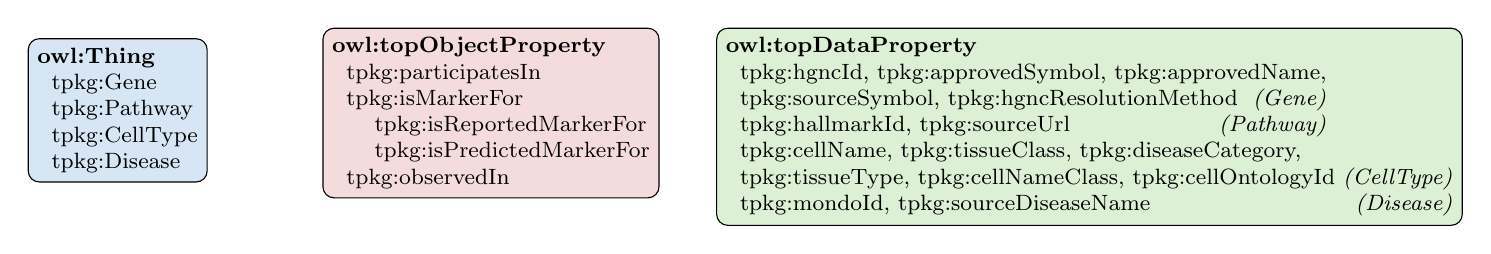
\begin{tikzpicture}[font=\footnotesize, every node/.style={align=left}]
  \node[draw, fill=ltloEtype, rounded corners] (cls) at (0,0) {\textbf{owl:Thing}\\
    \hspace{0.6em}tpkg:Gene\\ \hspace{0.6em}tpkg:Pathway\\ \hspace{0.6em}tpkg:CellType\\ \hspace{0.6em}tpkg:Disease};
  \node[draw, fill=ltloRel, rounded corners, anchor=north west] (op) at (2.6,1.05) {\textbf{owl:topObjectProperty}\\
    \hspace{0.6em}tpkg:participatesIn\\ \hspace{0.6em}tpkg:isMarkerFor\\ \hspace{1.8em}tpkg:isReportedMarkerFor\\ \hspace{1.8em}tpkg:isPredictedMarkerFor\\ \hspace{0.6em}tpkg:observedIn};
  \node[draw, fill=ltloAttr, rounded corners, anchor=north west] (dp) at (7.6,1.05) {\textbf{owl:topDataProperty}\\
    \hspace{0.6em}tpkg:hgncId, tpkg:approvedSymbol, tpkg:approvedName,\\ \hspace{0.6em}tpkg:sourceSymbol, tpkg:hgncResolutionMethod \hfill \emph{(Gene)}\\
    \hspace{0.6em}tpkg:hallmarkId, tpkg:sourceUrl \hfill \emph{(Pathway)}\\
    \hspace{0.6em}tpkg:cellName, tpkg:tissueClass, tpkg:diseaseCategory,\\ \hspace{0.6em}tpkg:tissueType, tpkg:cellNameClass, tpkg:cellOntologyId \hfill \emph{(CellType)}\\
    \hspace{0.6em}tpkg:mondoId, tpkg:sourceDiseaseName \hfill \emph{(Disease)}};
\end{tikzpicture}
\caption{Hierarchy of the language teleontology (classes, object properties, data properties)}
\label{fig:ltlo}
\end{figure}

\subsection{Data Layer}

The data layer aligns the datasets with the terms fixed above: columns that no concept defines are filtered out, the remaining ones are renamed to the language terms, and values are brought to the formats of their ranges. The raw files are never modified; every step is a script that writes new files, so the processed data can be rebuilt from the raw files (running the scripts twice gives identical files). Tests on small fixtures cover the gene resolution (13 tests) and the disease matching (12 tests); all pass. The decisions taken in this layer continue the numbering of Phase~1 and are collected in Table~\ref{tab:data-decisions}.

\subsubsection{Gene symbols: resolution against HGNC}

{\raggedright \noindent\textbf{Source files:} \texttt{h.all.v2026.2.Hs.symbols.gmt}, \texttt{human\_cell\_marker.txt}, \texttt{hgnc\_complete\_set.txt}.\\ \textbf{Script:} \texttt{hgnc\_resolution.py}.\\ \textbf{Output:} \texttt{gene\_symbol\_resolution.csv}, one row per distinct symbol per source.\par}

Every symbol is compared with the approved HGNC symbols using one normalization for all sources (trim, then upper case), which is only a matching key: the original spelling is kept. For CellMarker the gene is taken from \texttt{symbol} when it is filled and from \texttt{marker} otherwise. All 45,326 HGNC records have status \emph{Approved} and a well-formed identifier (\texttt{HGNC:n}). Table~\ref{tab:hgnc-resolution} gives the outcome.

\begin{table}[htbp]
\centering
\small
\begin{tabularx}{\linewidth}{|X|r|r|}
\hline
 & \textbf{MSigDB Hallmark} & \textbf{CellMarker 3.0} \\ \hline
Distinct symbols & 4,384 & 57,763 \\ \hline
Occurrences (gene--set pairs / records) & 7,322 & 1,779,944 \\ \hline
Resolved on the approved symbol & 4,383 & 30,615 \\ \hline
Resolved on a unique previous or alias symbol (D20) & 0 & 881 (11,557 records) \\ \hline
Previous/alias symbol with more than one candidate & 0 & 20 (67 records) \\ \hline
Not found & 1 (\emph{TARP}) & 25,952 (147,210 records) \\ \hline
Invalid (free text) & 0 & 295 (456 records) \\ \hline
\textbf{Kept in the KG (D21)} & \textbf{4,383 (7,321 occurrences)} & \textbf{31,496 (1,632,211 records, 91.7\%)} \\ \hline
\end{tabularx}
\caption{HGNC resolution of the gene symbols}
\label{tab:hgnc-resolution}
\end{table}

The CellMarker symbols that are not found come almost all from the \texttt{marker} column: clone and locus names such as \emph{AC092580.4}, and protein markers such as \emph{HLA-DR} or \emph{CD45RA}. Comparing the CellMarker \texttt{gene\_id} with the Entrez identifier in HGNC also showed that 3,774 resolved symbols (11,371 records) carry a \texttt{gene\_id} that is not the human one; almost all are written with mouse capitalization (e.g.\ \emph{A2m}), although the file labels every record as human (D19).

\subsubsection{MSigDB Hallmark}

{\raggedright \noindent\textbf{Source file:} \texttt{h.all.v2026.2.Hs.symbols.gmt}.\\ \textbf{Script:} \texttt{prepare\_msigdb.py}.\\ \textbf{Output:} \texttt{pathways.csv} (\texttt{hallmarkId}, \texttt{label}, \texttt{sourceUrl}) and \texttt{pathway\_gene.csv} (\texttt{hallmarkId}, \texttt{hgncId}, \texttt{sourceSymbol}).\par}
\begin{itemize}
    \item \textbf{Filtering:} all three fields of the file are used; only the gene without an HGNC identifier (\emph{TARP}) is dropped, so \texttt{HALLMARK\_ANDROGEN\_RESPONSE} goes from 101 to 100 genes.
    \item \textbf{Formatting:} the 50 identifiers have the form \texttt{HALLMARK\_...} and the 50 URLs start with \texttt{https://}. The file has no readable name, so the label is built from the identifier (D23): \texttt{HALLMARK\_TNFA\_SIGNALING\_VIA\_NFKB} $\rightarrow$ \emph{TNFA SIGNALING VIA NFKB}.
    \item \textbf{Result:} 50 pathways and 7,321 \texttt{participatesIn} links over 4,383 genes; pathway sizes stay between 32 and 200 genes.
\end{itemize}

\subsubsection{CellMarker 3.0}

{\raggedright \noindent\textbf{Source file:} \texttt{human\_cell\_marker.txt}.\\ \textbf{Script:} \texttt{prepare\_cellmarker.py}.\\ \textbf{Output:} \texttt{cell\_types.csv}, \texttt{cell\_type\_gene.csv} (the marker links with their kind) and \texttt{cell\_type\_disease\_source.csv} (input of the disease matching).\par}
\begin{itemize}
    \item \textbf{Filtering:} all 1,779,944 records are human (checked). Of the 23 columns we keep the cell name, tissue class, disease category, tissue type, cell name class, Cell Ontology identifier, disease, the gene (\texttt{symbol} or \texttt{marker}), and \texttt{marker\_source}, which is used only to choose between reported and predicted. The other columns (publication, year, method, series, UBERON identifier, \ldots) are not carried over.
    \item \textbf{Duplicates (D3):} 88,979 rows (5.0\%) are exact copies of another row and are collapsed, leaving 1,690,965 distinct records.
    \item \textbf{Renamed columns:} \texttt{cell\_name} $\rightarrow$ \texttt{cellName}, \texttt{tissue\_class} $\rightarrow$ \texttt{tissueClass}, \texttt{disease\_category} $\rightarrow$ \texttt{diseaseCategory}, \texttt{tissue\_type} $\rightarrow$ \texttt{tissueType}, \texttt{cell\_name\_class} $\rightarrow$ \texttt{cellNameClass}, \texttt{cellontology\_id} $\rightarrow$ \texttt{cellOntologyId}, \texttt{disease} $\rightarrow$ \texttt{sourceDiseaseName}.
    \item \textbf{Value formats:} 2,111 records write the CL identifier as \texttt{CL:nnnnnnn} and are changed to \texttt{CL\_nnnnnnn}; 14 distinct values (1,608 records) are not valid CL identifiers (UBERON identifiers or a wrong number of digits) and are treated as missing.
    \item \textbf{Checks:} every cell name has exactly one cell name class.
    \item \textbf{Result:} 12,632 CellTypes, of which 12,460 enter the KG (D22), and 873,776 \texttt{isMarkerFor} links over 26,886 genes: 101,897 reported and 771,879 predicted. In Phase~1 the same split, computed on the raw symbols before resolution, gave 977,460 links.
\end{itemize}

\subsubsection{Genes}

{\raggedright \noindent\textbf{Script:} \texttt{prepare\_genes.py}.\\ \textbf{Output:} \texttt{genes.csv} (\texttt{hgncId}, \texttt{approvedSymbol}, \texttt{approvedName}, \texttt{sourceSymbol}, \texttt{hgncResolutionMethod}).\par}
The KG has 26,893 genes: 4,376 in both sources (same HGNC identifier), 7 only in MSigDB and 22,510 only in CellMarker. 382 genes are reached only through a previous or alias symbol; 4,271 have more than one source spelling, all kept in \texttt{sourceSymbol}.

\subsubsection{Diseases: matching to MONDO}

{\raggedright \noindent\textbf{Source files:} \texttt{cell\_type\_disease\_source.csv}, \texttt{mondo.owl} (release 2026-11-03).\\ \textbf{Script:} \texttt{mondo\_matching.py}.\\ \textbf{Output:} \texttt{diseases.csv}, \texttt{cell\_type\_disease.csv} (the \texttt{observedIn} links) and the audit tables \texttt{disease\_mondo\_matching.csv} and \texttt{mondo\_merges.csv}.\par}

Both sides are normalized in the same way (lower case, \emph{tumour} $\rightarrow$ \emph{tumor}, possessive \emph{'s} removed, hyphens, underscores, commas and slashes turned into spaces). A disease string is resolved when exactly one non-obsolete MONDO term has it as label or EXACT synonym, on the full string or on the string without its final part in parentheses (\emph{Lung adenocarcinoma (LUAD)} $\rightarrow$ \emph{lung adenocarcinoma}). EXACT synonyms typed as abbreviations (or as ambiguous, dubious, deprecated or non-human) are not used, so an abbreviation alone never gives a match; RELATED, NARROW and BROAD synonyms are only recorded as candidates. Only resolved strings give a Disease and an \texttt{observedIn} link.

\begin{table}[htbp]
\centering
\small
\begin{tabularx}{\linewidth}{|X|r|r|}
\hline
\textbf{Outcome} & \textbf{Strings} & \textbf{Records} \\ \hline
Resolved (536 on the full string, 26 without the parentheses) & 562 & 554,287 (73.2\%) \\ \hline
Only a RELATED/NARROW/BROAD synonym & 20 & 10,220 (1.3\%) \\ \hline
Ambiguous (two human MONDO terms) & 2 & 11 \\ \hline
No match & 447 & 183,438 (24.2\%) \\ \hline
Not a disease (D14, D26) & 30 & 9,542 (1.3\%) \\ \hline
Merge rejected after review (D25) & 3 & 69 \\ \hline
\end{tabularx}
\caption{Matching of the 1,064 CellMarker disease strings of the KG CellTypes to MONDO}
\label{tab:mondo-matching}
\end{table}

The resolved strings give 517 Diseases and 10,254 \texttt{observedIn} links over 5,565 CellTypes. 37 MONDO terms are reached by more than one string (e.g.\ \emph{Gastric cancer}, \emph{Stomach cancer} and \emph{Gastric cancer (circulating)} $\rightarrow$ \emph{gastric cancer}); the original strings are kept in \texttt{sourceDiseaseName}. 1,429 of the 6,994 CellTypes with category Cancer or Disease have no \texttt{observedIn} link, because none of their disease strings is resolved. Of the 32 strings that mention a metastasis, 30 have no match and 2 (\emph{Metastatic melanoma}, \emph{Metastatic prostate cancer}) match a MONDO term of their own, so no metastasis is merged into its primary cancer.

\begin{table}[htbp]
\centering
\footnotesize
\begin{tabularx}{\linewidth}{|l|X|X|}
\hline
\textbf{ID} & \textbf{Question} & \textbf{Decision} \\ \hline
D3 & Exact duplicate rows in CellMarker? (open since Phase~1) & Collapsed and counted: the KG keeps no per-record data, so duplicates change no triple. \\ \hline
D19 & Resolved symbols whose CellMarker \texttt{gene\_id} is not the human one (mostly mouse-style symbols)? & Kept on the human gene, since the record is labelled human and the symbol matches; each case is flagged in the audit table. \\ \hline
D20 & Do we resolve previous and alias symbols? & Only with exactly one candidate, and the method is recorded (\texttt{hgncResolutionMethod}). \\ \hline
D21 & Genes that cannot be resolved? & Excluded from the KG; they stay in the audit table. \\ \hline
D22 & CellTypes left without any marker gene after D21? & Excluded (172 of 12,632). \\ \hline
D23 & How is the Pathway label built? & Identifier without \texttt{HALLMARK\_}, underscores turned into spaces, upper case kept (acronyms stay correct). \\ \hline
D24 & MONDO terms of non-human animal diseases? & Not used (8,319 terms under MONDO:0005583); otherwise \emph{Multiple myeloma} was ambiguous with its non-human-animal variant. \\ \hline
D25 & Review of the strings merged on the same MONDO term? & All accepted except three where the string is broader than the term (\emph{Primary antibody deficiency}, \emph{Lewy body disease}, \emph{Intervertebral disc disease}). \\ \hline
D26 & Completing the list of values that are not diseases (D14)? & 30 values: the 5 of Phase~1 plus ageing, exposures, viruses named as organisms, transplantation procedures, and study or state descriptions. None had a MONDO match. \\ \hline
\end{tabularx}
\caption{Decisions taken in the data layer}
\label{tab:data-decisions}
\end{table}

\subsection{Qualitative Evaluation}

\noindent\textbf{Entity type terms.} Initially considered: 4. Finally considered: 4. Aligned to the language teleontology: 4 (Table~\ref{tab:eval-etypes}).

\begin{table}[htbp]
\centering
\small
\begin{tabularx}{\linewidth}{|l|c|c|X|}
\hline
\textbf{Term} & \textbf{Initially?} & \textbf{Finally?} & \textbf{Alignment} \\ \hline
\texttt{tpkg:Gene} & Yes & Yes & UKC-29340 \emph{gene} \\ \hline
\texttt{tpkg:Pathway} & Yes & Yes & NCIT:C54214 \emph{Pathway} \\ \hline
\texttt{tpkg:CellType} & Yes & Yes & EFO:0000324 \emph{cell type} \\ \hline
\texttt{tpkg:Disease} & Yes & Yes & UKC-67092 \emph{disease} \\ \hline
\end{tabularx}
\caption{Entity type terms: definition and alignment}
\label{tab:eval-etypes}
\end{table}

\noindent\textbf{Object property terms.} Initially considered: 5. Finally considered: 5. Aligned to an existing concept: 2; the other 3 are new concepts (Table~\ref{tab:eval-oprops}).

\begin{table}[htbp]
\centering
\small
\begin{tabularx}{\linewidth}{|l|c|c|X|}
\hline
\textbf{Term} & \textbf{Initially?} & \textbf{Finally?} & \textbf{Alignment} \\ \hline
\texttt{tpkg:participatesIn} & Yes & Yes & RO:0000056 \emph{participates in} \\ \hline
\texttt{tpkg:isMarkerFor} & Yes & Yes & RO:0002607 \emph{is marker for} \\ \hline
\texttt{tpkg:isReportedMarkerFor} & Yes & Yes & New: TPKG26-01 \\ \hline
\texttt{tpkg:isPredictedMarkerFor} & Yes & Yes & New: TPKG26-02 \\ \hline
\texttt{tpkg:observedIn} & Yes & Yes & New: TPKG26-03 \\ \hline
\end{tabularx}
\caption{Object property terms: definition and alignment}
\label{tab:eval-oprops}
\end{table}

\noindent\textbf{Data property terms.} Initially considered: 21 (the 17 attributes of the Phase~1 ER model and the 4 evidence attributes removed at the end of Phase~1). Finally considered: 16 (the two labels become one term). Aligned to an existing concept: 12; the other 4 are new concepts (Table~\ref{tab:eval-dprops}).

\begin{table}[htbp]
\centering
\footnotesize
\begin{tabularx}{\linewidth}{|l|l|c|c|X|}
\hline
\textbf{Phase 1 term} & \textbf{Final term} & \textbf{Initially?} & \textbf{Finally?} & \textbf{Alignment} \\ \hline
HGNC ID & \texttt{tpkg:hgncId} & Yes & Yes & EDAM:data\_2298 \\ \hline
approved symbol & \texttt{tpkg:approvedSymbol} & Yes & Yes & NCIT:C43568 \\ \hline
approved name & \texttt{tpkg:approvedName} & Yes & Yes & EDAM:data\_2299 \\ \hline
source symbol(s) & \texttt{tpkg:sourceSymbol} & Yes & Yes & EDAM:data\_1026 \\ \hline
resolution status & \texttt{tpkg:hgncResolutionMethod} & Yes & Yes & New: TPKG26-04 \\ \hline
Hallmark identifier & \texttt{tpkg:hallmarkId} & Yes & Yes & EDAM:data\_1082 \\ \hline
label (Pathway) & \texttt{rdfs:label} & Yes & Yes & \texttt{rdfs:label} (merged with the Disease label) \\ \hline
source URL & \texttt{tpkg:sourceUrl} & Yes & Yes & EDAM:data\_1052 \\ \hline
cell name & \texttt{tpkg:cellName} & Yes & Yes & EDAM:data\_2892 \\ \hline
tissue class & \texttt{tpkg:tissueClass} & Yes & Yes & New: TPKG26-05 \\ \hline
disease category & \texttt{tpkg:diseaseCategory} & Yes & Yes & New: TPKG26-06 \\ \hline
tissue type & \texttt{tpkg:tissueType} & Yes & Yes & UKC-28479 \\ \hline
cell name class & \texttt{tpkg:cellNameClass} & Yes & Yes & New: TPKG26-07 \\ \hline
Cell Ontology ID & \texttt{tpkg:cellOntologyId} & Yes & Yes & EDAM:data\_3238 \\ \hline
MONDO ID & \texttt{tpkg:mondoId} & Yes & Yes & EDAM:data\_3667 \\ \hline
label (Disease) & \texttt{rdfs:label} & Yes & Yes & \texttt{rdfs:label} (merged with the Pathway label) \\ \hline
source strings & \texttt{tpkg:sourceDiseaseName} & Yes & Yes & EDAM:data\_3668 \\ \hline
marker source & -- & Yes & No & Removed in Phase~1; survives only as the choice of sub-property \\ \hline
method details & -- & Yes & No & Removed in Phase~1 \\ \hline
PubMed ID & -- & Yes & No & Removed in Phase~1 \\ \hline
publication year & -- & Yes & No & Removed in Phase~1 \\ \hline
\end{tabularx}
\caption{Data property terms: definition and alignment}
\label{tab:eval-dprops}
\end{table}

\noindent\textbf{Enrichment of the language teleontology.} Seven concepts were added (Table~\ref{tab:enrichment}). They cover what is specific to CellMarker or to our processing; each one is placed under the closest existing concept.

\begin{table}[htbp]
\centering
\footnotesize
\begin{tabularx}{\linewidth}{|l|l|X|}
\hline
\textbf{ID} & \textbf{Term} & \textbf{Parent concept and reason} \\ \hline
TPKG26-01 & is reported marker for & \texttt{tpkg:isMarkerFor}; the reported/predicted split decided in Phase~1 exists in no resource \\ \hline
TPKG26-02 & is predicted marker for & \texttt{tpkg:isMarkerFor}; as above \\ \hline
TPKG26-03 & observed in & UKC-105475 \emph{occur} (``to be found to exist''); the UKC verbs \emph{observe} have the active sense of someone observing \\ \hline
TPKG26-04 & HGNC resolution method & UKC-38540 \emph{result}; a property of our own processing \\ \hline
TPKG26-05 & tissue class & UKC-28479 \emph{tissue}; grouping defined by CellMarker (138 values) \\ \hline
TPKG26-06 & disease category & UKC-31356 \emph{category}; grouping defined by CellMarker (Normal, Cancer, Disease) \\ \hline
TPKG26-07 & cell name class & UKC-42808 \emph{class}; grouping defined by CellMarker (248 values) \\ \hline
\end{tabularx}
\caption{Concepts added to the language teleontology}
\label{tab:enrichment}
\end{table}

\noindent\textbf{Changes to the Purpose Definition.} Only one small change was made to Phase~1: the example of a pathway label, first given as \emph{Hypoxia}, was aligned to the rule D23 (\emph{HYPOXIA}) in the concept tables, the ER model and Section~3. Two questions that Phase~1 had left open were closed here: the duplicate rows (D3) and the list of values that are not diseases (D14, completed by D26). The Phase~1 figures that came from a prototype were recomputed on the real pipeline: 562 matched disease strings and 517 Diseases (the prototype gave 569 and 521), and 873,776 marker links after HGNC resolution (977,460 before).

\noindent\textbf{Dataset-level formatting and transformations.} They are described dataset by dataset in the data layer above. In summary, the processed data contain 26,893 genes, 50 pathways, 12,460 cell types and 517 diseases, with 7,321 \texttt{participatesIn}, 873,776 \texttt{isMarkerFor} (101,897 reported, 771,879 predicted) and 10,254 \texttt{observedIn} links. No gene lacks an approved name and no disease lacks a label; 164 cell types have no valid Cell Ontology identifier.

\noindent\textbf{Remarks on LLM usage.} LLMs were used in this phase (Appendix~A). The Claude Code agent was used, under our direction, to organize the Markdown files of the phase folder, to write and test the data-layer scripts, and to draft this documentation. Candidate concepts were looked up in the UKC and the biomedical ontologies interactively; every alignment, every custom concept and every data-layer decision (D3, D19--D26) was chosen by us, and every concept ID and gloss was checked on its source.

\noindent\textbf{The phase-specific LLM questionnaire is answered in Appendix A.}
